\documentclass[twoside]{book}

% Packages required by doxygen
\usepackage{fixltx2e}
\usepackage{calc}
\usepackage{doxygen}
\usepackage[export]{adjustbox} % also loads graphicx
\usepackage{graphicx}
\usepackage[utf8]{inputenc}
\usepackage{makeidx}
\usepackage{multicol}
\usepackage{multirow}
\PassOptionsToPackage{warn}{textcomp}
\usepackage{textcomp}
\usepackage[nointegrals]{wasysym}
\usepackage[table]{xcolor}

% Font selection
\usepackage[T1]{fontenc}
\usepackage[scaled=.90]{helvet}
\usepackage{courier}
\usepackage{amssymb}
\usepackage{sectsty}
\renewcommand{\familydefault}{\sfdefault}
\allsectionsfont{%
  \fontseries{bc}\selectfont%
  \color{darkgray}%
}
\renewcommand{\DoxyLabelFont}{%
  \fontseries{bc}\selectfont%
  \color{darkgray}%
}
\newcommand{\+}{\discretionary{\mbox{\scriptsize$\hookleftarrow$}}{}{}}

% Page & text layout
\usepackage{geometry}
\geometry{%
  a4paper,%
  top=2.5cm,%
  bottom=2.5cm,%
  left=2.5cm,%
  right=2.5cm%
}
\tolerance=750
\hfuzz=15pt
\hbadness=750
\setlength{\emergencystretch}{15pt}
\setlength{\parindent}{0cm}
\setlength{\parskip}{0.2cm}
\makeatletter
\renewcommand{\paragraph}{%
  \@startsection{paragraph}{4}{0ex}{-1.0ex}{1.0ex}{%
    \normalfont\normalsize\bfseries\SS@parafont%
  }%
}
\renewcommand{\subparagraph}{%
  \@startsection{subparagraph}{5}{0ex}{-1.0ex}{1.0ex}{%
    \normalfont\normalsize\bfseries\SS@subparafont%
  }%
}
\makeatother

% Headers & footers
\usepackage{fancyhdr}
\pagestyle{fancyplain}
\fancyhead[LE]{\fancyplain{}{\bfseries\thepage}}
\fancyhead[CE]{\fancyplain{}{}}
\fancyhead[RE]{\fancyplain{}{\bfseries\leftmark}}
\fancyhead[LO]{\fancyplain{}{\bfseries\rightmark}}
\fancyhead[CO]{\fancyplain{}{}}
\fancyhead[RO]{\fancyplain{}{\bfseries\thepage}}
\fancyfoot[LE]{\fancyplain{}{}}
\fancyfoot[CE]{\fancyplain{}{}}
\fancyfoot[RE]{\fancyplain{}{\bfseries\scriptsize Generated on Tue Dec 15 2015 15\+:48\+:03 for Flappy\+\_\+\+Bird by Doxygen }}
\fancyfoot[LO]{\fancyplain{}{\bfseries\scriptsize Generated on Tue Dec 15 2015 15\+:48\+:03 for Flappy\+\_\+\+Bird by Doxygen }}
\fancyfoot[CO]{\fancyplain{}{}}
\fancyfoot[RO]{\fancyplain{}{}}
\renewcommand{\footrulewidth}{0.4pt}
\renewcommand{\chaptermark}[1]{%
  \markboth{#1}{}%
}
\renewcommand{\sectionmark}[1]{%
  \markright{\thesection\ #1}%
}

% Indices & bibliography
\usepackage{natbib}
\usepackage[titles]{tocloft}
\setcounter{tocdepth}{3}
\setcounter{secnumdepth}{5}
\makeindex

% Hyperlinks (required, but should be loaded last)
\usepackage{ifpdf}
\ifpdf
  \usepackage[pdftex,pagebackref=true]{hyperref}
\else
  \usepackage[ps2pdf,pagebackref=true]{hyperref}
\fi
\hypersetup{%
  colorlinks=true,%
  linkcolor=blue,%
  citecolor=blue,%
  unicode%
}

% Custom commands
\newcommand{\clearemptydoublepage}{%
  \newpage{\pagestyle{empty}\cleardoublepage}%
}


%===== C O N T E N T S =====

\begin{document}

% Titlepage & ToC
\hypersetup{pageanchor=false,
             bookmarks=true,
             bookmarksnumbered=true,
             pdfencoding=unicode
            }
\pagenumbering{roman}
\begin{titlepage}
\vspace*{7cm}
\begin{center}%
{\Large Flappy\+\_\+\+Bird }\\
\vspace*{1cm}
{\large Generated by Doxygen 1.8.10}\\
\vspace*{0.5cm}
{\small Tue Dec 15 2015 15:48:03}\\
\end{center}
\end{titlepage}
\clearemptydoublepage
\tableofcontents
\clearemptydoublepage
\pagenumbering{arabic}
\hypersetup{pageanchor=true}

%--- Begin generated contents ---
\chapter{Namespace Index}
\section{Namespace List}
Here is a list of all documented namespaces with brief descriptions\+:\begin{DoxyCompactList}
\item\contentsline{section}{\hyperlink{namespace_ui}{Ui} }{\pageref{namespace_ui}}{}
\end{DoxyCompactList}

\chapter{Hierarchical Index}
\section{Class Hierarchy}
This inheritance list is sorted roughly, but not completely, alphabetically\+:\begin{DoxyCompactList}
\item \contentsline{section}{Game\+Level}{\pageref{class_game_level}}{}
\item Q\+Dialog\begin{DoxyCompactList}
\item \contentsline{section}{Difficulty\+Dialog}{\pageref{class_difficulty_dialog}}{}
\item \contentsline{section}{G\+O\+Dialog}{\pageref{class_g_o_dialog}}{}
\end{DoxyCompactList}
\item Q\+Graphics\+Scene\begin{DoxyCompactList}
\item \contentsline{section}{Main\+Scene}{\pageref{class_main_scene}}{}
\end{DoxyCompactList}
\item Q\+Main\+Window\begin{DoxyCompactList}
\item \contentsline{section}{Main\+Window}{\pageref{class_main_window}}{}
\end{DoxyCompactList}
\item Q\+Object\begin{DoxyCompactList}
\item \contentsline{section}{F\+B\+Helper}{\pageref{class_f_b_helper}}{}
\item \contentsline{section}{U\+I\+Controller}{\pageref{class_u_i_controller}}{}
\end{DoxyCompactList}
\end{DoxyCompactList}

\chapter{Class Index}
\section{Class List}
Here are the classes, structs, unions and interfaces with brief descriptions\+:\begin{DoxyCompactList}
\item\contentsline{section}{\hyperlink{class_difficulty_dialog}{Difficulty\+Dialog} }{\pageref{class_difficulty_dialog}}{}
\item\contentsline{section}{\hyperlink{class_f_b_helper}{F\+B\+Helper} }{\pageref{class_f_b_helper}}{}
\item\contentsline{section}{\hyperlink{class_game_level}{Game\+Level} \\*The \hyperlink{class_game_level}{Game\+Level} class }{\pageref{class_game_level}}{}
\item\contentsline{section}{\hyperlink{class_g_o_dialog}{G\+O\+Dialog} }{\pageref{class_g_o_dialog}}{}
\item\contentsline{section}{\hyperlink{class_main_scene}{Main\+Scene} \\*The \hyperlink{class_main_scene}{Main\+Scene} class This is the main graphics scene of the game It is used to manage all the moving items (the birds and flowers) as well as the background }{\pageref{class_main_scene}}{}
\item\contentsline{section}{\hyperlink{class_main_window}{Main\+Window} \\*This class handles the creating of the objects that are later controlled by the \hyperlink{class_main_scene}{Main\+Scene} class }{\pageref{class_main_window}}{}
\item\contentsline{section}{\hyperlink{class_u_i_controller}{U\+I\+Controller} \\*The Scene\+Controller class This is the primary controller of the G\+U\+I. It controls all the behaviors on the main window and its scene }{\pageref{class_u_i_controller}}{}
\end{DoxyCompactList}

\chapter{Namespace Documentation}
\hypertarget{namespace_ui}{}\section{Ui Namespace Reference}
\label{namespace_ui}\index{Ui@{Ui}}


\subsection{Detailed Description}
Opens the difficulty dialog box and gives speed and separation options. 
\chapter{Class Documentation}
\hypertarget{class_difficulty_dialog}{}\section{Difficulty\+Dialog Class Reference}
\label{class_difficulty_dialog}\index{Difficulty\+Dialog@{Difficulty\+Dialog}}
Inheritance diagram for Difficulty\+Dialog\+:\begin{figure}[H]
\begin{center}
\leavevmode
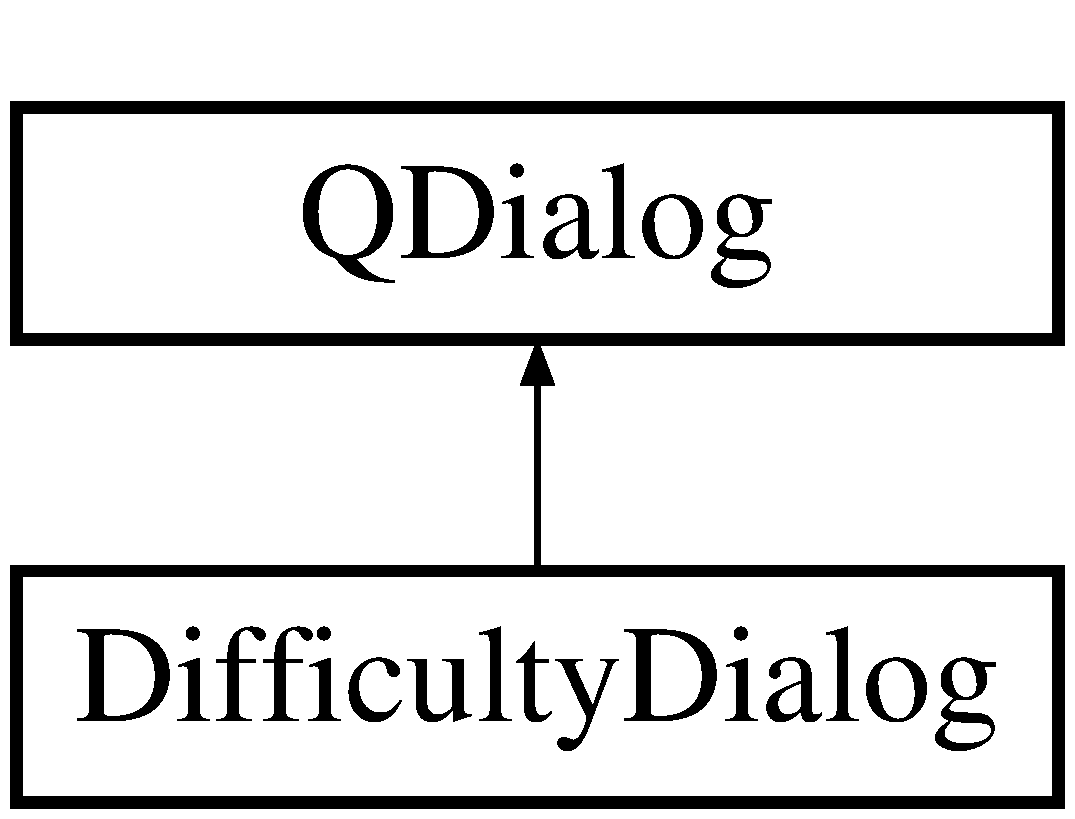
\includegraphics[height=2.000000cm]{class_difficulty_dialog}
\end{center}
\end{figure}
\subsection*{Signals}
\begin{DoxyCompactItemize}
\item 
\hypertarget{class_difficulty_dialog_a679aa2992b14e1d1d13d71b1811cd2da}{}void {\bfseries start\+Game} ()\label{class_difficulty_dialog_a679aa2992b14e1d1d13d71b1811cd2da}

\end{DoxyCompactItemize}
\subsection*{Public Member Functions}
\begin{DoxyCompactItemize}
\item 
\hyperlink{class_difficulty_dialog_a306929965fd40117b7ad8cff31cad0cf}{Difficulty\+Dialog} (Q\+Widget $\ast$parent=0)
\begin{DoxyCompactList}\small\item\em \hyperlink{class_difficulty_dialog_a306929965fd40117b7ad8cff31cad0cf}{Difficulty\+Dialog\+::\+Difficulty\+Dialog}. \end{DoxyCompactList}\item 
\hypertarget{class_difficulty_dialog_a5fc0e40c7c1460e2acdafbdbb0888614}{}\hyperlink{class_difficulty_dialog_a5fc0e40c7c1460e2acdafbdbb0888614}{$\sim$\+Difficulty\+Dialog} ()\label{class_difficulty_dialog_a5fc0e40c7c1460e2acdafbdbb0888614}

\begin{DoxyCompactList}\small\item\em \hyperlink{class_difficulty_dialog_a5fc0e40c7c1460e2acdafbdbb0888614}{Difficulty\+Dialog\+::$\sim$\+Difficulty\+Dialog}. \end{DoxyCompactList}\end{DoxyCompactItemize}
\subsection*{Protected Member Functions}
\begin{DoxyCompactItemize}
\item 
\hypertarget{class_difficulty_dialog_a84d7b9d77f578dd9626e254992abc91d}{}virtual void \hyperlink{class_difficulty_dialog_a84d7b9d77f578dd9626e254992abc91d}{close\+Event} (Q\+Close\+Event $\ast$)\label{class_difficulty_dialog_a84d7b9d77f578dd9626e254992abc91d}

\begin{DoxyCompactList}\small\item\em \hyperlink{class_difficulty_dialog_a84d7b9d77f578dd9626e254992abc91d}{Difficulty\+Dialog\+::close\+Event}. \end{DoxyCompactList}\end{DoxyCompactItemize}


\subsection{Constructor \& Destructor Documentation}
\hypertarget{class_difficulty_dialog_a306929965fd40117b7ad8cff31cad0cf}{}\index{Difficulty\+Dialog@{Difficulty\+Dialog}!Difficulty\+Dialog@{Difficulty\+Dialog}}
\index{Difficulty\+Dialog@{Difficulty\+Dialog}!Difficulty\+Dialog@{Difficulty\+Dialog}}
\subsubsection[{Difficulty\+Dialog(\+Q\+Widget $\ast$parent=0)}]{\setlength{\rightskip}{0pt plus 5cm}Difficulty\+Dialog\+::\+Difficulty\+Dialog (
\begin{DoxyParamCaption}
\item[{Q\+Widget $\ast$}]{parent = {\ttfamily 0}}
\end{DoxyParamCaption}
)\hspace{0.3cm}{\ttfamily [explicit]}}\label{class_difficulty_dialog_a306929965fd40117b7ad8cff31cad0cf}


\hyperlink{class_difficulty_dialog_a306929965fd40117b7ad8cff31cad0cf}{Difficulty\+Dialog\+::\+Difficulty\+Dialog}. 


\begin{DoxyParams}{Parameters}
{\em parent} & \\
\hline
\end{DoxyParams}


The documentation for this class was generated from the following files\+:\begin{DoxyCompactItemize}
\item 
difficultydialog.\+h\item 
difficultydialog.\+cpp\end{DoxyCompactItemize}

\hypertarget{class_f_b_helper}{}\section{F\+B\+Helper Class Reference}
\label{class_f_b_helper}\index{F\+B\+Helper@{F\+B\+Helper}}


{\ttfamily \#include $<$fbhelper.\+h$>$}

Inheritance diagram for F\+B\+Helper\+:\begin{figure}[H]
\begin{center}
\leavevmode
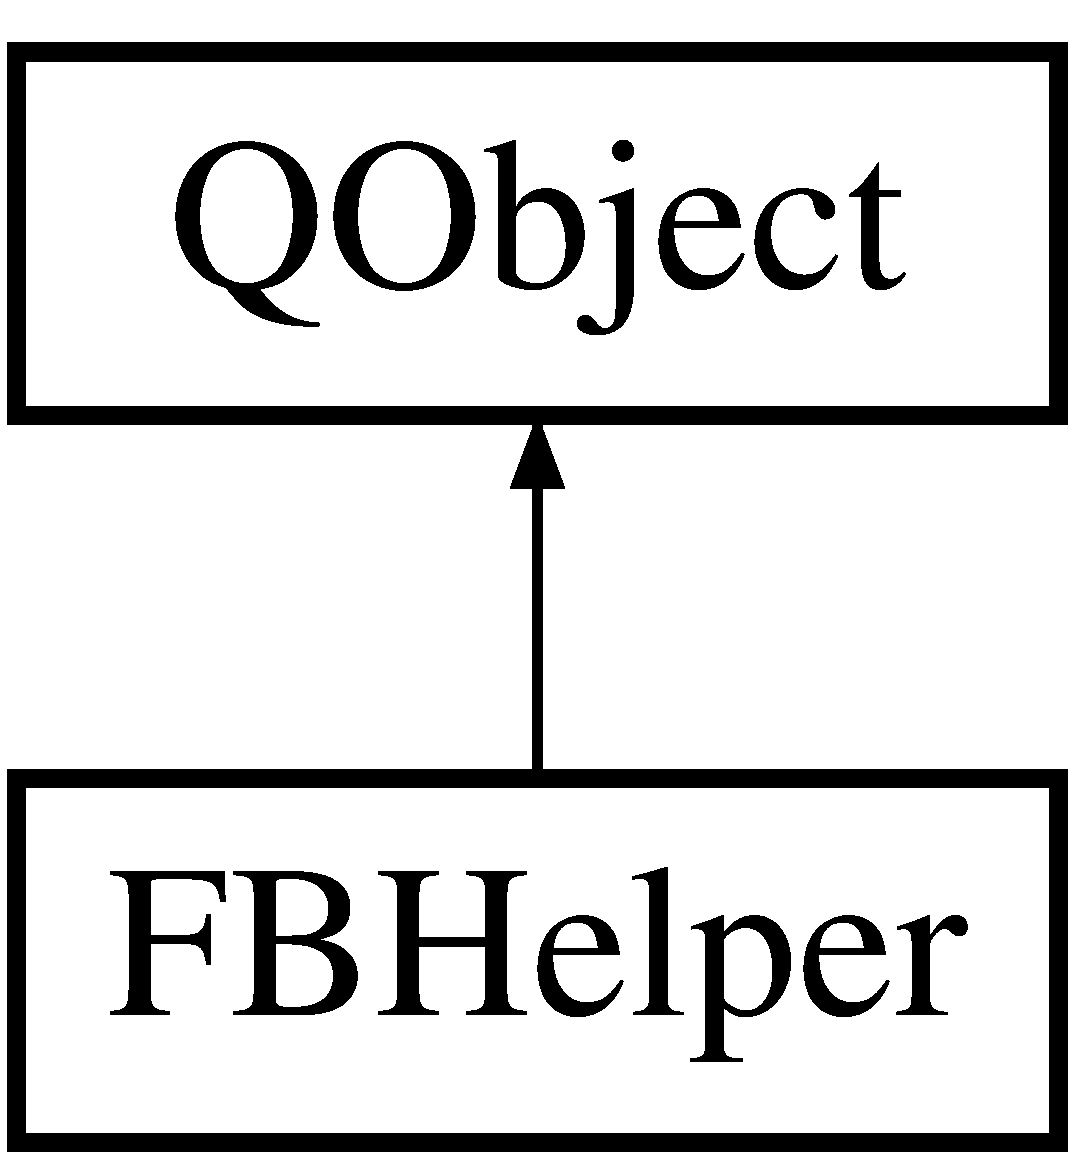
\includegraphics[height=2.000000cm]{class_f_b_helper}
\end{center}
\end{figure}
\subsection*{Public Member Functions}
\begin{DoxyCompactItemize}
\item 
\hypertarget{class_f_b_helper_a2cb5a6e986f1c155861d6327535ddadd}{}\hyperlink{class_f_b_helper_a2cb5a6e986f1c155861d6327535ddadd}{F\+B\+Helper} ()\label{class_f_b_helper_a2cb5a6e986f1c155861d6327535ddadd}

\begin{DoxyCompactList}\small\item\em \hyperlink{class_f_b_helper_a2cb5a6e986f1c155861d6327535ddadd}{F\+B\+Helper\+::\+F\+B\+Helper}. \end{DoxyCompactList}\item 
void \hyperlink{class_f_b_helper_afc18a55cac693f74248d2d3b9d4b2347}{save} (Q\+String user\+Name, int score)
\begin{DoxyCompactList}\small\item\em \hyperlink{class_f_b_helper_afc18a55cac693f74248d2d3b9d4b2347}{F\+B\+Helper\+::save}. \end{DoxyCompactList}\end{DoxyCompactItemize}


\subsection{Detailed Description}
The Flapping Bird Helper class. 

\subsection{Member Function Documentation}
\hypertarget{class_f_b_helper_afc18a55cac693f74248d2d3b9d4b2347}{}\index{F\+B\+Helper@{F\+B\+Helper}!save@{save}}
\index{save@{save}!F\+B\+Helper@{F\+B\+Helper}}
\subsubsection[{save(\+Q\+String user\+Name, int score)}]{\setlength{\rightskip}{0pt plus 5cm}void F\+B\+Helper\+::save (
\begin{DoxyParamCaption}
\item[{Q\+String}]{user\+Name, }
\item[{int}]{score}
\end{DoxyParamCaption}
)}\label{class_f_b_helper_afc18a55cac693f74248d2d3b9d4b2347}


\hyperlink{class_f_b_helper_afc18a55cac693f74248d2d3b9d4b2347}{F\+B\+Helper\+::save}. 


\begin{DoxyParams}{Parameters}
{\em user\+Name} & \\
\hline
{\em score} & \\
\hline
\end{DoxyParams}
\begin{DoxyReturn}{Returns}

\end{DoxyReturn}


The documentation for this class was generated from the following files\+:\begin{DoxyCompactItemize}
\item 
fbhelper.\+h\item 
fbhelper.\+cpp\end{DoxyCompactItemize}

\hypertarget{class_game_level}{}\section{Game\+Level Class Reference}
\label{class_game_level}\index{Game\+Level@{Game\+Level}}


The \hyperlink{class_game_level}{Game\+Level} class.  




{\ttfamily \#include $<$gamelevel.\+h$>$}

\subsection*{Public Member Functions}
\begin{DoxyCompactItemize}
\item 
Q\+String \hyperlink{class_game_level_acab80c7bfab374236d1a5bd55a10ff7e}{get\+Level\+N} () const 
\begin{DoxyCompactList}\small\item\em \hyperlink{class_game_level_acab80c7bfab374236d1a5bd55a10ff7e}{Game\+Level\+::get\+Level\+N}. \end{DoxyCompactList}\item 
int \hyperlink{class_game_level_a5e06760f7b73f987f6fbb42f9a7ff89f}{get\+Id} () const 
\begin{DoxyCompactList}\small\item\em \hyperlink{class_game_level_a5e06760f7b73f987f6fbb42f9a7ff89f}{Game\+Level\+::get\+Id}. \end{DoxyCompactList}\end{DoxyCompactItemize}
\subsection*{Static Public Member Functions}
\begin{DoxyCompactItemize}
\item 
static void \hyperlink{class_game_level_aecafb8ea53d8fbc0c354db3e7b877848}{set\+Level\+N} (const Q\+String \&value)
\begin{DoxyCompactList}\small\item\em \hyperlink{class_game_level_aecafb8ea53d8fbc0c354db3e7b877848}{Game\+Level\+::set\+Level\+N}. \end{DoxyCompactList}\item 
static void \hyperlink{class_game_level_a15dbe223c7d2d2cf22bf869c44b7cc35}{set\+Id} (int value)
\begin{DoxyCompactList}\small\item\em \hyperlink{class_game_level_a15dbe223c7d2d2cf22bf869c44b7cc35}{Game\+Level\+::set\+Id}. \end{DoxyCompactList}\item 
static \hyperlink{class_game_level}{Game\+Level} \hyperlink{class_game_level_abfd8683983588ee8343b26e194d493ac}{get\+Instance} ()
\begin{DoxyCompactList}\small\item\em Game\+Level\+::get\+G\+Level. \end{DoxyCompactList}\item 
static float \hyperlink{class_game_level_a3bad525afd79aa4653538b360e5b053d}{get\+Bird\+Pic\+Scalar} ()
\begin{DoxyCompactList}\small\item\em \hyperlink{class_game_level_a3bad525afd79aa4653538b360e5b053d}{Game\+Level\+::get\+Bird\+Pic\+Scalar}. \end{DoxyCompactList}\item 
static int \hyperlink{class_game_level_a9a15dd2831a62009c270eb9d7669a9d9}{get\+Flower\+Speed} ()
\begin{DoxyCompactList}\small\item\em \hyperlink{class_game_level_a9a15dd2831a62009c270eb9d7669a9d9}{Game\+Level\+::get\+Flower\+Speed}. \end{DoxyCompactList}\end{DoxyCompactItemize}
\subsection*{Static Public Attributes}
\begin{DoxyCompactItemize}
\item 
static const \hyperlink{class_game_level}{Game\+Level} \hyperlink{class_game_level_a4de2cb0a8609b8e9a76f64a1502a71de}{E\+A\+S\+Y}
\begin{DoxyCompactList}\small\item\em \hyperlink{class_game_level_a4de2cb0a8609b8e9a76f64a1502a71de}{Game\+Level\+::\+E\+A\+S\+Y}. \end{DoxyCompactList}\item 
\hypertarget{class_game_level_aaf2d9c7c8b6b88817451aa23442477c9}{}static const \hyperlink{class_game_level}{Game\+Level} \hyperlink{class_game_level_aaf2d9c7c8b6b88817451aa23442477c9}{M\+E\+D\+I\+U\+M}\label{class_game_level_aaf2d9c7c8b6b88817451aa23442477c9}

\begin{DoxyCompactList}\small\item\em \hyperlink{class_game_level_aaf2d9c7c8b6b88817451aa23442477c9}{Game\+Level\+::\+M\+E\+D\+I\+U\+M}. \end{DoxyCompactList}\item 
\hypertarget{class_game_level_adec4e386d38dfb062e733098696524a7}{}static const \hyperlink{class_game_level}{Game\+Level} \hyperlink{class_game_level_adec4e386d38dfb062e733098696524a7}{H\+A\+R\+D}\label{class_game_level_adec4e386d38dfb062e733098696524a7}

\begin{DoxyCompactList}\small\item\em \hyperlink{class_game_level_adec4e386d38dfb062e733098696524a7}{Game\+Level\+::\+H\+A\+R\+D}. \end{DoxyCompactList}\end{DoxyCompactItemize}


\subsection{Detailed Description}
The \hyperlink{class_game_level}{Game\+Level} class. 

This class is implemented in form of combination of singleton and type-\/safe enum design patterns. It is used for managing the difficuty of a game , and the difficulty is defined base on the bird size and the flower speed. The class is simultaneously accessed by all U\+I components. 

\subsection{Member Function Documentation}
\hypertarget{class_game_level_a3bad525afd79aa4653538b360e5b053d}{}\index{Game\+Level@{Game\+Level}!get\+Bird\+Pic\+Scalar@{get\+Bird\+Pic\+Scalar}}
\index{get\+Bird\+Pic\+Scalar@{get\+Bird\+Pic\+Scalar}!Game\+Level@{Game\+Level}}
\subsubsection[{get\+Bird\+Pic\+Scalar()}]{\setlength{\rightskip}{0pt plus 5cm}float Game\+Level\+::get\+Bird\+Pic\+Scalar (
\begin{DoxyParamCaption}
{}
\end{DoxyParamCaption}
)\hspace{0.3cm}{\ttfamily [static]}}\label{class_game_level_a3bad525afd79aa4653538b360e5b053d}


\hyperlink{class_game_level_a3bad525afd79aa4653538b360e5b053d}{Game\+Level\+::get\+Bird\+Pic\+Scalar}. 

\begin{DoxyReturn}{Returns}

\end{DoxyReturn}
\hypertarget{class_game_level_a9a15dd2831a62009c270eb9d7669a9d9}{}\index{Game\+Level@{Game\+Level}!get\+Flower\+Speed@{get\+Flower\+Speed}}
\index{get\+Flower\+Speed@{get\+Flower\+Speed}!Game\+Level@{Game\+Level}}
\subsubsection[{get\+Flower\+Speed()}]{\setlength{\rightskip}{0pt plus 5cm}int Game\+Level\+::get\+Flower\+Speed (
\begin{DoxyParamCaption}
{}
\end{DoxyParamCaption}
)\hspace{0.3cm}{\ttfamily [static]}}\label{class_game_level_a9a15dd2831a62009c270eb9d7669a9d9}


\hyperlink{class_game_level_a9a15dd2831a62009c270eb9d7669a9d9}{Game\+Level\+::get\+Flower\+Speed}. 

\begin{DoxyReturn}{Returns}

\end{DoxyReturn}
\hypertarget{class_game_level_a5e06760f7b73f987f6fbb42f9a7ff89f}{}\index{Game\+Level@{Game\+Level}!get\+Id@{get\+Id}}
\index{get\+Id@{get\+Id}!Game\+Level@{Game\+Level}}
\subsubsection[{get\+Id() const }]{\setlength{\rightskip}{0pt plus 5cm}int Game\+Level\+::get\+Id (
\begin{DoxyParamCaption}
{}
\end{DoxyParamCaption}
) const}\label{class_game_level_a5e06760f7b73f987f6fbb42f9a7ff89f}


\hyperlink{class_game_level_a5e06760f7b73f987f6fbb42f9a7ff89f}{Game\+Level\+::get\+Id}. 

\begin{DoxyReturn}{Returns}

\end{DoxyReturn}
\hypertarget{class_game_level_abfd8683983588ee8343b26e194d493ac}{}\index{Game\+Level@{Game\+Level}!get\+Instance@{get\+Instance}}
\index{get\+Instance@{get\+Instance}!Game\+Level@{Game\+Level}}
\subsubsection[{get\+Instance()}]{\setlength{\rightskip}{0pt plus 5cm}{\bf Game\+Level} Game\+Level\+::get\+Instance (
\begin{DoxyParamCaption}
{}
\end{DoxyParamCaption}
)\hspace{0.3cm}{\ttfamily [static]}}\label{class_game_level_abfd8683983588ee8343b26e194d493ac}


Game\+Level\+::get\+G\+Level. 

The singleton method \begin{DoxyReturn}{Returns}

\end{DoxyReturn}
\hypertarget{class_game_level_acab80c7bfab374236d1a5bd55a10ff7e}{}\index{Game\+Level@{Game\+Level}!get\+Level\+N@{get\+Level\+N}}
\index{get\+Level\+N@{get\+Level\+N}!Game\+Level@{Game\+Level}}
\subsubsection[{get\+Level\+N() const }]{\setlength{\rightskip}{0pt plus 5cm}Q\+String Game\+Level\+::get\+Level\+N (
\begin{DoxyParamCaption}
{}
\end{DoxyParamCaption}
) const}\label{class_game_level_acab80c7bfab374236d1a5bd55a10ff7e}


\hyperlink{class_game_level_acab80c7bfab374236d1a5bd55a10ff7e}{Game\+Level\+::get\+Level\+N}. 

\begin{DoxyReturn}{Returns}

\end{DoxyReturn}
\hypertarget{class_game_level_a15dbe223c7d2d2cf22bf869c44b7cc35}{}\index{Game\+Level@{Game\+Level}!set\+Id@{set\+Id}}
\index{set\+Id@{set\+Id}!Game\+Level@{Game\+Level}}
\subsubsection[{set\+Id(int value)}]{\setlength{\rightskip}{0pt plus 5cm}void Game\+Level\+::set\+Id (
\begin{DoxyParamCaption}
\item[{int}]{value}
\end{DoxyParamCaption}
)\hspace{0.3cm}{\ttfamily [static]}}\label{class_game_level_a15dbe223c7d2d2cf22bf869c44b7cc35}


\hyperlink{class_game_level_a15dbe223c7d2d2cf22bf869c44b7cc35}{Game\+Level\+::set\+Id}. 


\begin{DoxyParams}{Parameters}
{\em value} & \\
\hline
\end{DoxyParams}
\hypertarget{class_game_level_aecafb8ea53d8fbc0c354db3e7b877848}{}\index{Game\+Level@{Game\+Level}!set\+Level\+N@{set\+Level\+N}}
\index{set\+Level\+N@{set\+Level\+N}!Game\+Level@{Game\+Level}}
\subsubsection[{set\+Level\+N(const Q\+String \&value)}]{\setlength{\rightskip}{0pt plus 5cm}void Game\+Level\+::set\+Level\+N (
\begin{DoxyParamCaption}
\item[{const Q\+String \&}]{value}
\end{DoxyParamCaption}
)\hspace{0.3cm}{\ttfamily [static]}}\label{class_game_level_aecafb8ea53d8fbc0c354db3e7b877848}


\hyperlink{class_game_level_aecafb8ea53d8fbc0c354db3e7b877848}{Game\+Level\+::set\+Level\+N}. 


\begin{DoxyParams}{Parameters}
{\em value} & \\
\hline
\end{DoxyParams}


\subsection{Member Data Documentation}
\hypertarget{class_game_level_a4de2cb0a8609b8e9a76f64a1502a71de}{}\index{Game\+Level@{Game\+Level}!E\+A\+S\+Y@{E\+A\+S\+Y}}
\index{E\+A\+S\+Y@{E\+A\+S\+Y}!Game\+Level@{Game\+Level}}
\subsubsection[{E\+A\+S\+Y}]{\setlength{\rightskip}{0pt plus 5cm}{\bf Game\+Level} const Game\+Level\+::\+E\+A\+S\+Y\hspace{0.3cm}{\ttfamily [static]}}\label{class_game_level_a4de2cb0a8609b8e9a76f64a1502a71de}


\hyperlink{class_game_level_a4de2cb0a8609b8e9a76f64a1502a71de}{Game\+Level\+::\+E\+A\+S\+Y}. 

Reference to the function declaration 

The documentation for this class was generated from the following files\+:\begin{DoxyCompactItemize}
\item 
gamelevel.\+h\item 
gamelevel.\+cpp\end{DoxyCompactItemize}

\hypertarget{class_g_o_dialog}{}\section{G\+O\+Dialog Class Reference}
\label{class_g_o_dialog}\index{G\+O\+Dialog@{G\+O\+Dialog}}


{\ttfamily \#include $<$godialog.\+h$>$}

Inheritance diagram for G\+O\+Dialog\+:\begin{figure}[H]
\begin{center}
\leavevmode
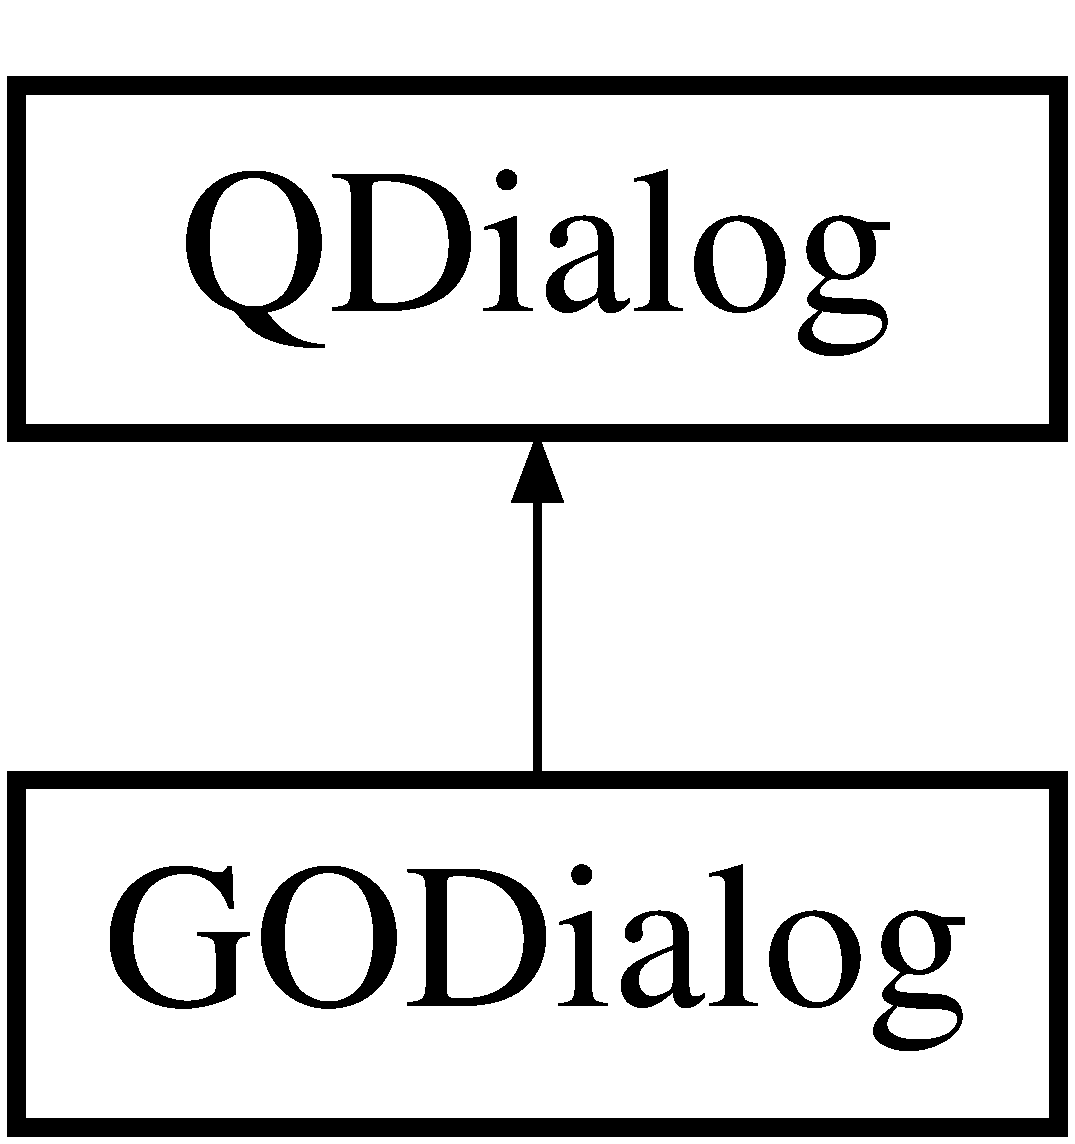
\includegraphics[height=2.000000cm]{class_g_o_dialog}
\end{center}
\end{figure}
\subsection*{Signals}
\begin{DoxyCompactItemize}
\item 
\hypertarget{class_g_o_dialog_ade3251194e62f4cd11d51deaa6d14ff8}{}void {\bfseries restart} ()\label{class_g_o_dialog_ade3251194e62f4cd11d51deaa6d14ff8}

\end{DoxyCompactItemize}
\subsection*{Public Member Functions}
\begin{DoxyCompactItemize}
\item 
\hyperlink{class_g_o_dialog_afd3447c4a8b2cd74b548cfb4b6828229}{G\+O\+Dialog} (Q\+Widget $\ast$parent=0)
\begin{DoxyCompactList}\small\item\em \hyperlink{class_g_o_dialog_afd3447c4a8b2cd74b548cfb4b6828229}{G\+O\+Dialog\+::\+G\+O\+Dialog}. \end{DoxyCompactList}\item 
\hypertarget{class_g_o_dialog_a1c2216da8ff22e04956fa0169829f3c1}{}\hyperlink{class_g_o_dialog_a1c2216da8ff22e04956fa0169829f3c1}{$\sim$\+G\+O\+Dialog} ()\label{class_g_o_dialog_a1c2216da8ff22e04956fa0169829f3c1}

\begin{DoxyCompactList}\small\item\em \hyperlink{class_g_o_dialog_a1c2216da8ff22e04956fa0169829f3c1}{G\+O\+Dialog\+::$\sim$\+G\+O\+Dialog}. \end{DoxyCompactList}\item 
void \hyperlink{class_g_o_dialog_aa3da50f6ca7030ce844c8207e4ba1bd7}{populate\+U\+I} (int score)
\begin{DoxyCompactList}\small\item\em G\+O\+Dialog\+::show. \end{DoxyCompactList}\end{DoxyCompactItemize}
\subsection*{Protected Member Functions}
\begin{DoxyCompactItemize}
\item 
\hypertarget{class_g_o_dialog_aefbba611da74930ee77c505b08e8f87a}{}virtual void \hyperlink{class_g_o_dialog_aefbba611da74930ee77c505b08e8f87a}{close\+Event} (Q\+Close\+Event $\ast$)\label{class_g_o_dialog_aefbba611da74930ee77c505b08e8f87a}

\begin{DoxyCompactList}\small\item\em \hyperlink{class_g_o_dialog_aefbba611da74930ee77c505b08e8f87a}{G\+O\+Dialog\+::close\+Event}. \end{DoxyCompactList}\end{DoxyCompactItemize}


\subsection{Detailed Description}
The game-\/over dialog. It has options to save to the R\+C\+C server 

\subsection{Constructor \& Destructor Documentation}
\hypertarget{class_g_o_dialog_afd3447c4a8b2cd74b548cfb4b6828229}{}\index{G\+O\+Dialog@{G\+O\+Dialog}!G\+O\+Dialog@{G\+O\+Dialog}}
\index{G\+O\+Dialog@{G\+O\+Dialog}!G\+O\+Dialog@{G\+O\+Dialog}}
\subsubsection[{G\+O\+Dialog(\+Q\+Widget $\ast$parent=0)}]{\setlength{\rightskip}{0pt plus 5cm}G\+O\+Dialog\+::\+G\+O\+Dialog (
\begin{DoxyParamCaption}
\item[{Q\+Widget $\ast$}]{parent = {\ttfamily 0}}
\end{DoxyParamCaption}
)\hspace{0.3cm}{\ttfamily [explicit]}}\label{class_g_o_dialog_afd3447c4a8b2cd74b548cfb4b6828229}


\hyperlink{class_g_o_dialog_afd3447c4a8b2cd74b548cfb4b6828229}{G\+O\+Dialog\+::\+G\+O\+Dialog}. 


\begin{DoxyParams}{Parameters}
{\em parent} & \\
\hline
\end{DoxyParams}


\subsection{Member Function Documentation}
\hypertarget{class_g_o_dialog_aa3da50f6ca7030ce844c8207e4ba1bd7}{}\index{G\+O\+Dialog@{G\+O\+Dialog}!populate\+U\+I@{populate\+U\+I}}
\index{populate\+U\+I@{populate\+U\+I}!G\+O\+Dialog@{G\+O\+Dialog}}
\subsubsection[{populate\+U\+I(int score)}]{\setlength{\rightskip}{0pt plus 5cm}void G\+O\+Dialog\+::populate\+U\+I (
\begin{DoxyParamCaption}
\item[{int}]{score}
\end{DoxyParamCaption}
)}\label{class_g_o_dialog_aa3da50f6ca7030ce844c8207e4ba1bd7}


G\+O\+Dialog\+::show. 


\begin{DoxyParams}{Parameters}
{\em score} & \\
\hline
\end{DoxyParams}


The documentation for this class was generated from the following files\+:\begin{DoxyCompactItemize}
\item 
godialog.\+h\item 
godialog.\+cpp\end{DoxyCompactItemize}

\hypertarget{class_main_scene}{}\section{Main\+Scene Class Reference}
\label{class_main_scene}\index{Main\+Scene@{Main\+Scene}}


The \hyperlink{class_main_scene}{Main\+Scene} class This is the main graphics scene of the game It is used to manage all the moving items (the birds and flowers) as well as the background.  




{\ttfamily \#include $<$mainscene.\+h$>$}

Inheritance diagram for Main\+Scene\+:\begin{figure}[H]
\begin{center}
\leavevmode
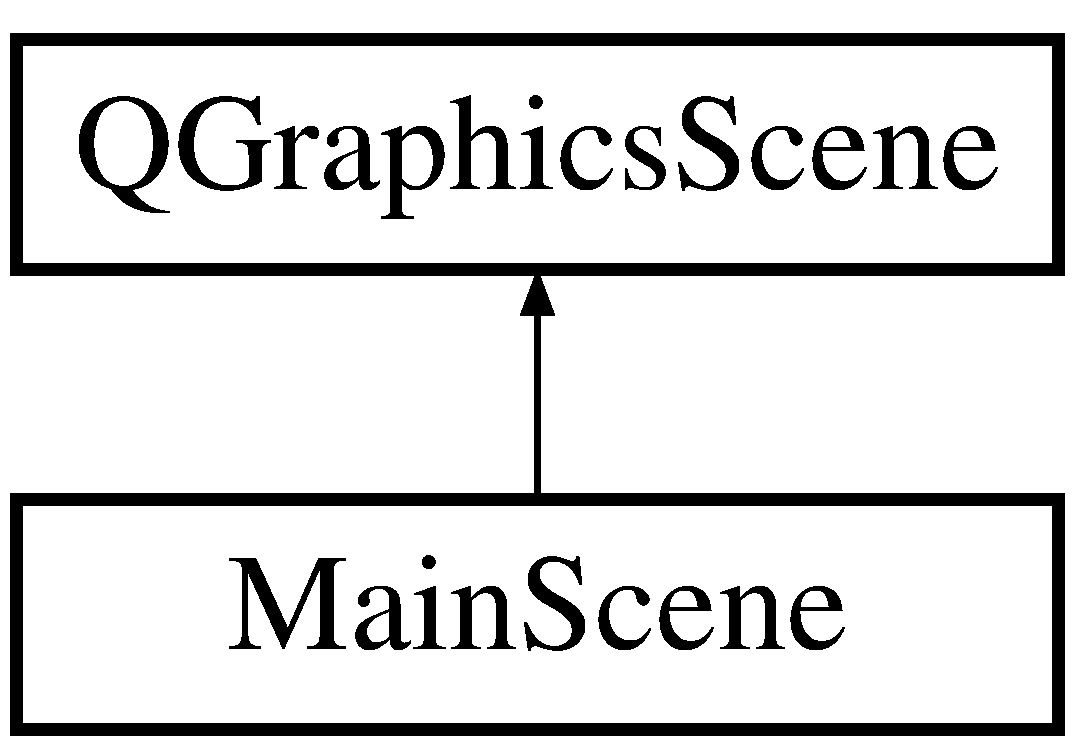
\includegraphics[height=2.000000cm]{class_main_scene}
\end{center}
\end{figure}
\subsection*{Public Member Functions}
\begin{DoxyCompactItemize}
\item 
\hyperlink{class_main_scene_a539e1c90b1c7f2e910d44cfd8ec45e1c}{Main\+Scene} (Q\+Object $\ast$parent=0)
\begin{DoxyCompactList}\small\item\em \hyperlink{class_main_scene_a539e1c90b1c7f2e910d44cfd8ec45e1c}{Main\+Scene\+::\+Main\+Scene}. \end{DoxyCompactList}\item 
void \hyperlink{class_main_scene_a204ffd620222634956a901d7cbc39a14}{create\+Flowers} ()
\begin{DoxyCompactList}\small\item\em \hyperlink{class_main_scene_a204ffd620222634956a901d7cbc39a14}{Main\+Scene\+::create\+Flowers}. \end{DoxyCompactList}\item 
void \hyperlink{class_main_scene_a34c634cb6edca409b8818b90a6c8f6a3}{move\+Flowers} ()
\begin{DoxyCompactList}\small\item\em \hyperlink{class_main_scene_a34c634cb6edca409b8818b90a6c8f6a3}{Main\+Scene\+::move\+Flowers}. \end{DoxyCompactList}\item 
void \hyperlink{class_main_scene_a9686cf85301e0adf9fdf6fcfac8e1d54}{play} ()
\begin{DoxyCompactList}\small\item\em \hyperlink{class_main_scene_a9686cf85301e0adf9fdf6fcfac8e1d54}{Main\+Scene\+::play}. \end{DoxyCompactList}\item 
void \hyperlink{class_main_scene_a2da7b3de66fab703d85ab25aa899f12b}{free\+Fall\+Bird} ()
\begin{DoxyCompactList}\small\item\em \hyperlink{class_main_scene_a2da7b3de66fab703d85ab25aa899f12b}{Main\+Scene\+::free\+Fall\+Bird}. \end{DoxyCompactList}\item 
void \hyperlink{class_main_scene_a61958a11669a25126ac32ac70a758c11}{fly\+Up\+Bird} ()
\begin{DoxyCompactList}\small\item\em \hyperlink{class_main_scene_a61958a11669a25126ac32ac70a758c11}{Main\+Scene\+::fly\+Up\+Bird}. \end{DoxyCompactList}\item 
bool \hyperlink{class_main_scene_a4b2d78977f11b426c324f66277546360}{has\+Collision} ()
\begin{DoxyCompactList}\small\item\em \hyperlink{class_main_scene_a4b2d78977f11b426c324f66277546360}{Main\+Scene\+::has\+Collision}. \end{DoxyCompactList}\item 
void \hyperlink{class_main_scene_a415d733af1f33b9af9f94042083472aa}{check\+For\+Collision} ()
\begin{DoxyCompactList}\small\item\em \hyperlink{class_main_scene_a415d733af1f33b9af9f94042083472aa}{Main\+Scene\+::check\+For\+Collision}. \end{DoxyCompactList}\item 
\hypertarget{class_main_scene_ab5f3fb8e1e0b77b63231ea976fe1eb25}{}void \hyperlink{class_main_scene_ab5f3fb8e1e0b77b63231ea976fe1eb25}{restart\+Scene} ()\label{class_main_scene_ab5f3fb8e1e0b77b63231ea976fe1eb25}

\begin{DoxyCompactList}\small\item\em \hyperlink{class_main_scene_ab5f3fb8e1e0b77b63231ea976fe1eb25}{Main\+Scene\+::restart\+Scene}. \end{DoxyCompactList}\end{DoxyCompactItemize}
\subsection*{Protected Member Functions}
\begin{DoxyCompactItemize}
\item 
void \hyperlink{class_main_scene_a8ba16fde46c54c2fa4098d03c9ffd332}{draw\+Background} (Q\+Painter $\ast$painter, const Q\+Rect\+F \&rect)
\begin{DoxyCompactList}\small\item\em draw\+Background \end{DoxyCompactList}\end{DoxyCompactItemize}


\subsection{Detailed Description}
The \hyperlink{class_main_scene}{Main\+Scene} class This is the main graphics scene of the game It is used to manage all the moving items (the birds and flowers) as well as the background. 

Authors\+: Hoa Huynh, Abel Salazar, Tiffany Pan 

\subsection{Constructor \& Destructor Documentation}
\hypertarget{class_main_scene_a539e1c90b1c7f2e910d44cfd8ec45e1c}{}\index{Main\+Scene@{Main\+Scene}!Main\+Scene@{Main\+Scene}}
\index{Main\+Scene@{Main\+Scene}!Main\+Scene@{Main\+Scene}}
\subsubsection[{Main\+Scene(\+Q\+Object $\ast$parent=0)}]{\setlength{\rightskip}{0pt plus 5cm}Main\+Scene\+::\+Main\+Scene (
\begin{DoxyParamCaption}
\item[{Q\+Object $\ast$}]{parent = {\ttfamily 0}}
\end{DoxyParamCaption}
)}\label{class_main_scene_a539e1c90b1c7f2e910d44cfd8ec45e1c}


\hyperlink{class_main_scene_a539e1c90b1c7f2e910d44cfd8ec45e1c}{Main\+Scene\+::\+Main\+Scene}. 

The main constructor is uesed for initating all components in this scene

Reference to the declaration of this constructor 
\begin{DoxyParams}{Parameters}
{\em parent} & \\
\hline
\end{DoxyParams}


\subsection{Member Function Documentation}
\hypertarget{class_main_scene_a415d733af1f33b9af9f94042083472aa}{}\index{Main\+Scene@{Main\+Scene}!check\+For\+Collision@{check\+For\+Collision}}
\index{check\+For\+Collision@{check\+For\+Collision}!Main\+Scene@{Main\+Scene}}
\subsubsection[{check\+For\+Collision()}]{\setlength{\rightskip}{0pt plus 5cm}void Main\+Scene\+::check\+For\+Collision (
\begin{DoxyParamCaption}
{}
\end{DoxyParamCaption}
)}\label{class_main_scene_a415d733af1f33b9af9f94042083472aa}


\hyperlink{class_main_scene_a415d733af1f33b9af9f94042083472aa}{Main\+Scene\+::check\+For\+Collision}. 

Reference to the declaration of this function \hypertarget{class_main_scene_a204ffd620222634956a901d7cbc39a14}{}\index{Main\+Scene@{Main\+Scene}!create\+Flowers@{create\+Flowers}}
\index{create\+Flowers@{create\+Flowers}!Main\+Scene@{Main\+Scene}}
\subsubsection[{create\+Flowers()}]{\setlength{\rightskip}{0pt plus 5cm}void Main\+Scene\+::create\+Flowers (
\begin{DoxyParamCaption}
{}
\end{DoxyParamCaption}
)}\label{class_main_scene_a204ffd620222634956a901d7cbc39a14}


\hyperlink{class_main_scene_a204ffd620222634956a901d7cbc39a14}{Main\+Scene\+::create\+Flowers}. 

Reference to the declaration of this function \hypertarget{class_main_scene_a8ba16fde46c54c2fa4098d03c9ffd332}{}\index{Main\+Scene@{Main\+Scene}!draw\+Background@{draw\+Background}}
\index{draw\+Background@{draw\+Background}!Main\+Scene@{Main\+Scene}}
\subsubsection[{draw\+Background(\+Q\+Painter $\ast$painter, const Q\+Rect\+F \&rect)}]{\setlength{\rightskip}{0pt plus 5cm}void Main\+Scene\+::draw\+Background (
\begin{DoxyParamCaption}
\item[{Q\+Painter $\ast$}]{painter, }
\item[{const Q\+Rect\+F \&}]{rect}
\end{DoxyParamCaption}
)\hspace{0.3cm}{\ttfamily [protected]}}\label{class_main_scene_a8ba16fde46c54c2fa4098d03c9ffd332}


draw\+Background 

\hyperlink{class_main_scene_a8ba16fde46c54c2fa4098d03c9ffd332}{Main\+Scene\+::draw\+Background}.

Overriding function from Q\+Graphics\+Scene This function will draw the background being one of three layers of the scene 
\begin{DoxyParams}{Parameters}
{\em painter} & \\
\hline
{\em rect} & Reference to the declaration of this function \\
\hline
{\em painter} & \\
\hline
{\em rect} & \\
\hline
\end{DoxyParams}
\hypertarget{class_main_scene_a61958a11669a25126ac32ac70a758c11}{}\index{Main\+Scene@{Main\+Scene}!fly\+Up\+Bird@{fly\+Up\+Bird}}
\index{fly\+Up\+Bird@{fly\+Up\+Bird}!Main\+Scene@{Main\+Scene}}
\subsubsection[{fly\+Up\+Bird()}]{\setlength{\rightskip}{0pt plus 5cm}void Main\+Scene\+::fly\+Up\+Bird (
\begin{DoxyParamCaption}
{}
\end{DoxyParamCaption}
)}\label{class_main_scene_a61958a11669a25126ac32ac70a758c11}


\hyperlink{class_main_scene_a61958a11669a25126ac32ac70a758c11}{Main\+Scene\+::fly\+Up\+Bird}. 

Reference to the declaration of this function \hypertarget{class_main_scene_a2da7b3de66fab703d85ab25aa899f12b}{}\index{Main\+Scene@{Main\+Scene}!free\+Fall\+Bird@{free\+Fall\+Bird}}
\index{free\+Fall\+Bird@{free\+Fall\+Bird}!Main\+Scene@{Main\+Scene}}
\subsubsection[{free\+Fall\+Bird()}]{\setlength{\rightskip}{0pt plus 5cm}void Main\+Scene\+::free\+Fall\+Bird (
\begin{DoxyParamCaption}
{}
\end{DoxyParamCaption}
)}\label{class_main_scene_a2da7b3de66fab703d85ab25aa899f12b}


\hyperlink{class_main_scene_a2da7b3de66fab703d85ab25aa899f12b}{Main\+Scene\+::free\+Fall\+Bird}. 

Reference to the declaration of this function \hypertarget{class_main_scene_a4b2d78977f11b426c324f66277546360}{}\index{Main\+Scene@{Main\+Scene}!has\+Collision@{has\+Collision}}
\index{has\+Collision@{has\+Collision}!Main\+Scene@{Main\+Scene}}
\subsubsection[{has\+Collision()}]{\setlength{\rightskip}{0pt plus 5cm}bool Main\+Scene\+::has\+Collision (
\begin{DoxyParamCaption}
{}
\end{DoxyParamCaption}
)}\label{class_main_scene_a4b2d78977f11b426c324f66277546360}


\hyperlink{class_main_scene_a4b2d78977f11b426c324f66277546360}{Main\+Scene\+::has\+Collision}. 

Reference to the declaration of this function \begin{DoxyReturn}{Returns}

\end{DoxyReturn}
\hypertarget{class_main_scene_a34c634cb6edca409b8818b90a6c8f6a3}{}\index{Main\+Scene@{Main\+Scene}!move\+Flowers@{move\+Flowers}}
\index{move\+Flowers@{move\+Flowers}!Main\+Scene@{Main\+Scene}}
\subsubsection[{move\+Flowers()}]{\setlength{\rightskip}{0pt plus 5cm}void Main\+Scene\+::move\+Flowers (
\begin{DoxyParamCaption}
{}
\end{DoxyParamCaption}
)}\label{class_main_scene_a34c634cb6edca409b8818b90a6c8f6a3}


\hyperlink{class_main_scene_a34c634cb6edca409b8818b90a6c8f6a3}{Main\+Scene\+::move\+Flowers}. 

Reference to the declaration of this function \hypertarget{class_main_scene_a9686cf85301e0adf9fdf6fcfac8e1d54}{}\index{Main\+Scene@{Main\+Scene}!play@{play}}
\index{play@{play}!Main\+Scene@{Main\+Scene}}
\subsubsection[{play()}]{\setlength{\rightskip}{0pt plus 5cm}void Main\+Scene\+::play (
\begin{DoxyParamCaption}
{}
\end{DoxyParamCaption}
)}\label{class_main_scene_a9686cf85301e0adf9fdf6fcfac8e1d54}


\hyperlink{class_main_scene_a9686cf85301e0adf9fdf6fcfac8e1d54}{Main\+Scene\+::play}. 

Reference to the declaration of this function 

The documentation for this class was generated from the following files\+:\begin{DoxyCompactItemize}
\item 
mainscene.\+h\item 
mainscene.\+cpp\end{DoxyCompactItemize}

\hypertarget{class_main_window}{}\section{Main\+Window Class Reference}
\label{class_main_window}\index{Main\+Window@{Main\+Window}}


This class handles the creating of the objects that are later controlled by the \hyperlink{class_main_scene}{Main\+Scene} class.  




{\ttfamily \#include $<$mainwindow.\+h$>$}

Inheritance diagram for Main\+Window\+:\begin{figure}[H]
\begin{center}
\leavevmode
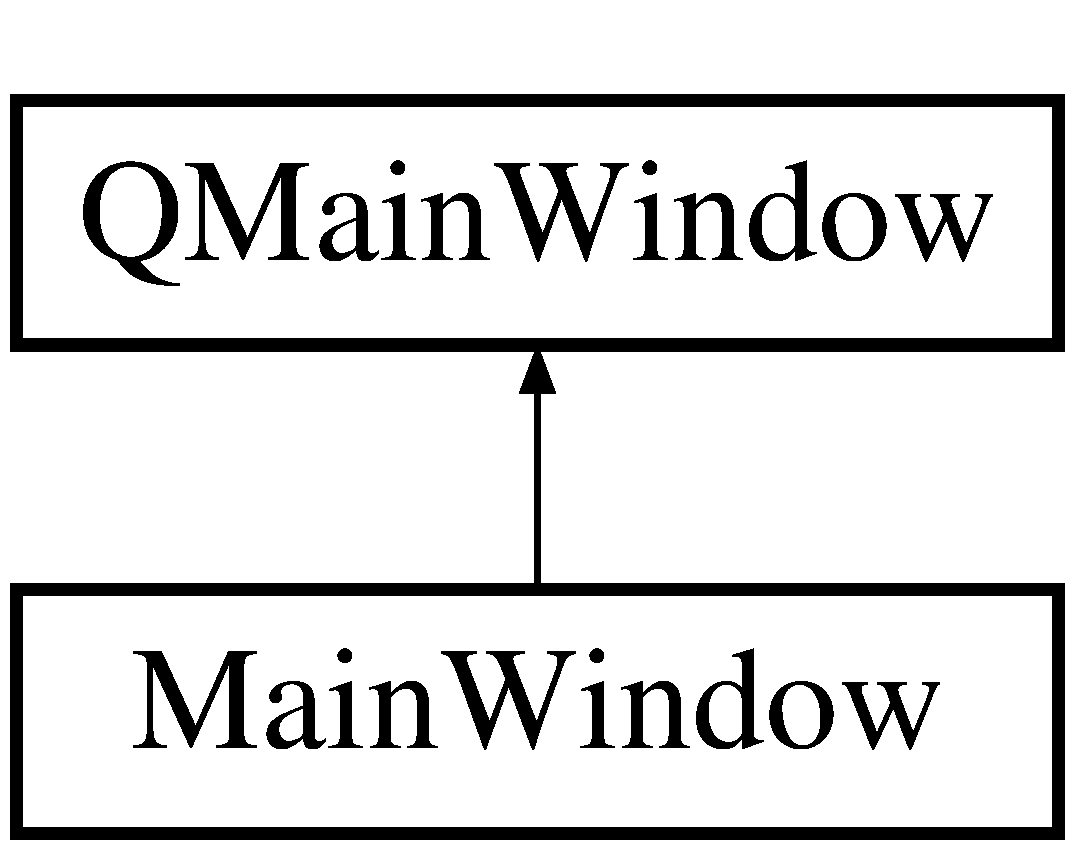
\includegraphics[height=2.000000cm]{class_main_window}
\end{center}
\end{figure}
\subsection*{Public Slots}
\begin{DoxyCompactItemize}
\item 
\hypertarget{class_main_window_a8f689d74e00fe7de42c89f81c5b63794}{}void {\bfseries move\+Flowers} ()\label{class_main_window_a8f689d74e00fe7de42c89f81c5b63794}

\item 
\hypertarget{class_main_window_a18e7270dcf1bcfe932068a1d2b7297d3}{}void {\bfseries free\+Fall\+Bird} ()\label{class_main_window_a18e7270dcf1bcfe932068a1d2b7297d3}

\end{DoxyCompactItemize}
\subsection*{Signals}
\begin{DoxyCompactItemize}
\item 
\hypertarget{class_main_window_aefc37cf67a2394c55485e6ccceedd612}{}void {\bfseries press\+Space\+Key} ()\label{class_main_window_aefc37cf67a2394c55485e6ccceedd612}

\item 
\hypertarget{class_main_window_a99aa56cd57bddd8bc91c3aa86a2d86a0}{}void {\bfseries process\+Collision} ()\label{class_main_window_a99aa56cd57bddd8bc91c3aa86a2d86a0}

\item 
\hypertarget{class_main_window_add1be06e623d9ca240573631e8b452dc}{}void {\bfseries level\+Up} ()\label{class_main_window_add1be06e623d9ca240573631e8b452dc}

\end{DoxyCompactItemize}
\subsection*{Public Member Functions}
\begin{DoxyCompactItemize}
\item 
\hypertarget{class_main_window_a8b244be8b7b7db1b08de2a2acb9409db}{}{\bfseries Main\+Window} (Q\+Widget $\ast$parent=0)\label{class_main_window_a8b244be8b7b7db1b08de2a2acb9409db}

\item 
\hypertarget{class_main_window_afc7af89bdb376772f2d61dec19ae1f82}{}void {\bfseries create\+Flowers} ()\label{class_main_window_afc7af89bdb376772f2d61dec19ae1f82}

\item 
\hypertarget{class_main_window_a4f035b25b6181829a9275155e3ca9bbd}{}void {\bfseries play} ()\label{class_main_window_a4f035b25b6181829a9275155e3ca9bbd}

\item 
\hypertarget{class_main_window_afa31474b493ee6d8847fdd6cbafd88a2}{}void {\bfseries fly\+Up\+Bird} ()\label{class_main_window_afa31474b493ee6d8847fdd6cbafd88a2}

\item 
\hypertarget{class_main_window_ac433c09c359ac237755e2266c4e0f76c}{}void {\bfseries update\+Score} ()\label{class_main_window_ac433c09c359ac237755e2266c4e0f76c}

\item 
\hypertarget{class_main_window_a4f4f4c634d8d1d1e46059ba7dd5648c6}{}int {\bfseries get\+Cr\+Score} () const \label{class_main_window_a4f4f4c634d8d1d1e46059ba7dd5648c6}

\item 
\hypertarget{class_main_window_a01a798332112e079bb1afab732318fb1}{}void \hyperlink{class_main_window_a01a798332112e079bb1afab732318fb1}{restart\+U\+I} ()\label{class_main_window_a01a798332112e079bb1afab732318fb1}

\begin{DoxyCompactList}\small\item\em \hyperlink{class_main_window_a01a798332112e079bb1afab732318fb1}{Main\+Window\+::restart\+U\+I}. \end{DoxyCompactList}\end{DoxyCompactItemize}
\subsection*{Protected Member Functions}
\begin{DoxyCompactItemize}
\item 
\hypertarget{class_main_window_a9c4f542263838b9ecd06eae839a42a34}{}void {\bfseries key\+Press\+Event} (Q\+Key\+Event $\ast$event)\label{class_main_window_a9c4f542263838b9ecd06eae839a42a34}

\end{DoxyCompactItemize}


\subsection{Detailed Description}
This class handles the creating of the objects that are later controlled by the \hyperlink{class_main_scene}{Main\+Scene} class. 

The documentation for this class was generated from the following files\+:\begin{DoxyCompactItemize}
\item 
mainwindow.\+h\item 
mainwindow.\+cpp\end{DoxyCompactItemize}

\hypertarget{class_u_i_controller}{}\section{U\+I\+Controller Class Reference}
\label{class_u_i_controller}\index{U\+I\+Controller@{U\+I\+Controller}}


The Scene\+Controller class This is the primary controller of the G\+U\+I. It controls all the behaviors on the main window and its scene.  




{\ttfamily \#include $<$uicontroller.\+h$>$}

Inheritance diagram for U\+I\+Controller\+:\begin{figure}[H]
\begin{center}
\leavevmode
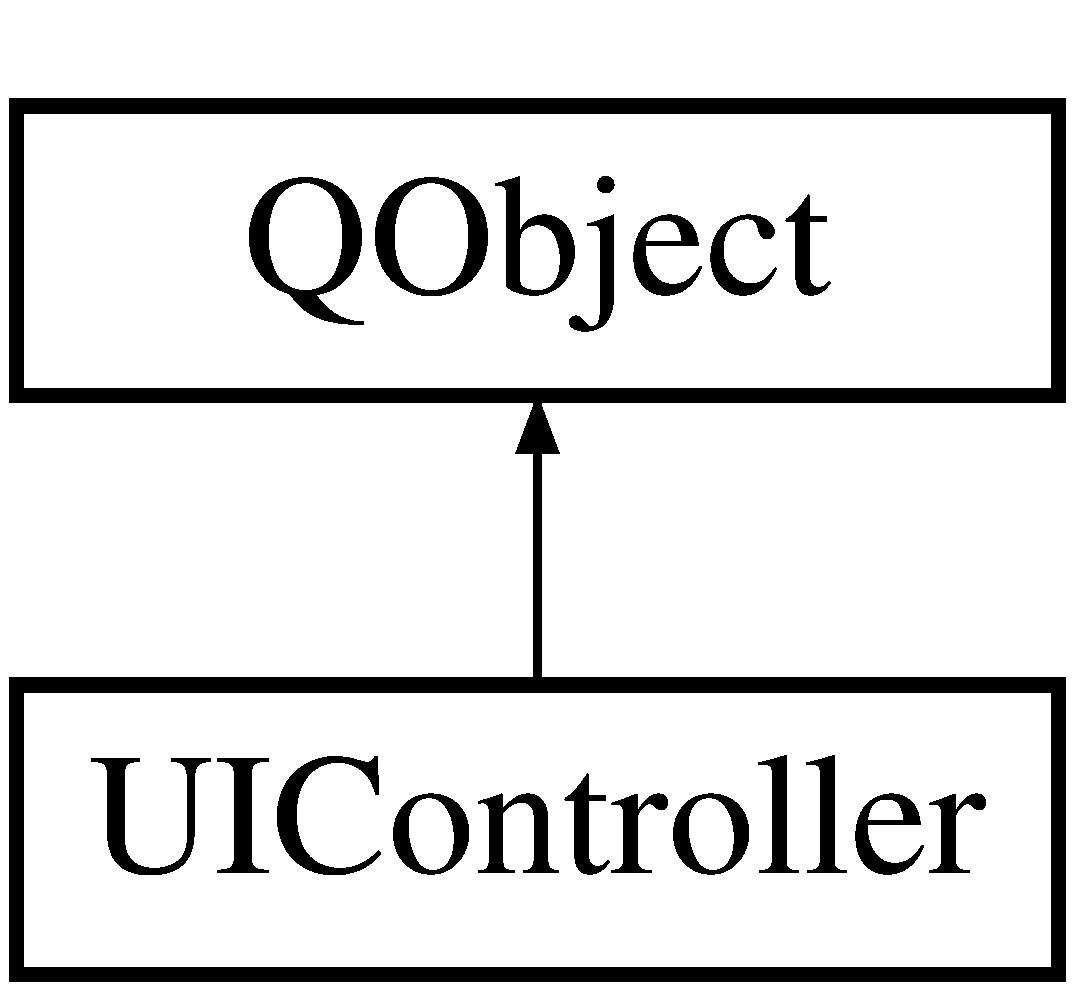
\includegraphics[height=2.000000cm]{class_u_i_controller}
\end{center}
\end{figure}
\subsection*{Public Slots}
\begin{DoxyCompactItemize}
\item 
void \hyperlink{class_u_i_controller_af487d6f8eb4913362bf2c3ddce1d402b}{create\+Flowers} ()
\begin{DoxyCompactList}\small\item\em U\+I\+Controller\+::create\+New\+F\+Lowers. \end{DoxyCompactList}\item 
void \hyperlink{class_u_i_controller_a99978cb677cdab656e0a5ad2b7409eb1}{process\+Space\+Key\+Press} ()
\begin{DoxyCompactList}\small\item\em U\+I\+Controller\+::process\+Key\+Press. \end{DoxyCompactList}\item 
void \hyperlink{class_u_i_controller_a265e9f0a72982a8b09b5e32087da469c}{process\+Collision} ()
\begin{DoxyCompactList}\small\item\em \hyperlink{class_u_i_controller_a265e9f0a72982a8b09b5e32087da469c}{U\+I\+Controller\+::process\+Collision}. \end{DoxyCompactList}\item 
void \hyperlink{class_u_i_controller_ac0b8e708ff0eb1a85c2714e137323e7f}{state\+Changed} (Q\+Media\+Player\+::\+State new\+State)
\begin{DoxyCompactList}\small\item\em \hyperlink{class_u_i_controller_ac0b8e708ff0eb1a85c2714e137323e7f}{U\+I\+Controller\+::state\+Changed}. \end{DoxyCompactList}\item 
void \hyperlink{class_u_i_controller_a5dafae54703cfe08050b2276c5770649}{start\+Game} ()
\begin{DoxyCompactList}\small\item\em \hyperlink{class_u_i_controller_a5dafae54703cfe08050b2276c5770649}{U\+I\+Controller\+::start\+Game}. \end{DoxyCompactList}\item 
void \hyperlink{class_u_i_controller_acee3e71fd6075cc4023df24562ce4fe4}{restart} ()
\begin{DoxyCompactList}\small\item\em \hyperlink{class_u_i_controller_acee3e71fd6075cc4023df24562ce4fe4}{U\+I\+Controller\+::restart}. \end{DoxyCompactList}\item 
void \hyperlink{class_u_i_controller_a612ce6f697961c095a491686f2210b77}{level\+Up} ()
\begin{DoxyCompactList}\small\item\em \hyperlink{class_u_i_controller_a612ce6f697961c095a491686f2210b77}{U\+I\+Controller\+::level\+Up}. \end{DoxyCompactList}\end{DoxyCompactItemize}
\subsection*{Public Member Functions}
\begin{DoxyCompactItemize}
\item 
\hyperlink{class_u_i_controller_a2057465975a34faaff5e07c77f0f63cd}{U\+I\+Controller} (Q\+Object $\ast$parent=0)
\begin{DoxyCompactList}\small\item\em \hyperlink{class_u_i_controller_a2057465975a34faaff5e07c77f0f63cd}{U\+I\+Controller\+::\+U\+I\+Controller}. \end{DoxyCompactList}\end{DoxyCompactItemize}


\subsection{Detailed Description}
The Scene\+Controller class This is the primary controller of the G\+U\+I. It controls all the behaviors on the main window and its scene. 

\subsection{Constructor \& Destructor Documentation}
\hypertarget{class_u_i_controller_a2057465975a34faaff5e07c77f0f63cd}{}\index{U\+I\+Controller@{U\+I\+Controller}!U\+I\+Controller@{U\+I\+Controller}}
\index{U\+I\+Controller@{U\+I\+Controller}!U\+I\+Controller@{U\+I\+Controller}}
\subsubsection[{U\+I\+Controller(\+Q\+Object $\ast$parent=0)}]{\setlength{\rightskip}{0pt plus 5cm}U\+I\+Controller\+::\+U\+I\+Controller (
\begin{DoxyParamCaption}
\item[{Q\+Object $\ast$}]{parent = {\ttfamily 0}}
\end{DoxyParamCaption}
)\hspace{0.3cm}{\ttfamily [explicit]}}\label{class_u_i_controller_a2057465975a34faaff5e07c77f0f63cd}


\hyperlink{class_u_i_controller_a2057465975a34faaff5e07c77f0f63cd}{U\+I\+Controller\+::\+U\+I\+Controller}. 

Reference to the function declaration 
\begin{DoxyParams}{Parameters}
{\em parent} & \\
\hline
\end{DoxyParams}


\subsection{Member Function Documentation}
\hypertarget{class_u_i_controller_af487d6f8eb4913362bf2c3ddce1d402b}{}\index{U\+I\+Controller@{U\+I\+Controller}!create\+Flowers@{create\+Flowers}}
\index{create\+Flowers@{create\+Flowers}!U\+I\+Controller@{U\+I\+Controller}}
\subsubsection[{create\+Flowers}]{\setlength{\rightskip}{0pt plus 5cm}void U\+I\+Controller\+::create\+Flowers (
\begin{DoxyParamCaption}
{}
\end{DoxyParamCaption}
)\hspace{0.3cm}{\ttfamily [slot]}}\label{class_u_i_controller_af487d6f8eb4913362bf2c3ddce1d402b}


U\+I\+Controller\+::create\+New\+F\+Lowers. 

Reference to the function declaration \hypertarget{class_u_i_controller_a612ce6f697961c095a491686f2210b77}{}\index{U\+I\+Controller@{U\+I\+Controller}!level\+Up@{level\+Up}}
\index{level\+Up@{level\+Up}!U\+I\+Controller@{U\+I\+Controller}}
\subsubsection[{level\+Up}]{\setlength{\rightskip}{0pt plus 5cm}void U\+I\+Controller\+::level\+Up (
\begin{DoxyParamCaption}
{}
\end{DoxyParamCaption}
)\hspace{0.3cm}{\ttfamily [slot]}}\label{class_u_i_controller_a612ce6f697961c095a491686f2210b77}


\hyperlink{class_u_i_controller_a612ce6f697961c095a491686f2210b77}{U\+I\+Controller\+::level\+Up}. 

Reference to the function declaration \hypertarget{class_u_i_controller_a265e9f0a72982a8b09b5e32087da469c}{}\index{U\+I\+Controller@{U\+I\+Controller}!process\+Collision@{process\+Collision}}
\index{process\+Collision@{process\+Collision}!U\+I\+Controller@{U\+I\+Controller}}
\subsubsection[{process\+Collision}]{\setlength{\rightskip}{0pt plus 5cm}void U\+I\+Controller\+::process\+Collision (
\begin{DoxyParamCaption}
{}
\end{DoxyParamCaption}
)\hspace{0.3cm}{\ttfamily [slot]}}\label{class_u_i_controller_a265e9f0a72982a8b09b5e32087da469c}


\hyperlink{class_u_i_controller_a265e9f0a72982a8b09b5e32087da469c}{U\+I\+Controller\+::process\+Collision}. 

Reference to the function declaration \hypertarget{class_u_i_controller_a99978cb677cdab656e0a5ad2b7409eb1}{}\index{U\+I\+Controller@{U\+I\+Controller}!process\+Space\+Key\+Press@{process\+Space\+Key\+Press}}
\index{process\+Space\+Key\+Press@{process\+Space\+Key\+Press}!U\+I\+Controller@{U\+I\+Controller}}
\subsubsection[{process\+Space\+Key\+Press}]{\setlength{\rightskip}{0pt plus 5cm}void U\+I\+Controller\+::process\+Space\+Key\+Press (
\begin{DoxyParamCaption}
{}
\end{DoxyParamCaption}
)\hspace{0.3cm}{\ttfamily [slot]}}\label{class_u_i_controller_a99978cb677cdab656e0a5ad2b7409eb1}


U\+I\+Controller\+::process\+Key\+Press. 

Reference to the function declaration \hypertarget{class_u_i_controller_acee3e71fd6075cc4023df24562ce4fe4}{}\index{U\+I\+Controller@{U\+I\+Controller}!restart@{restart}}
\index{restart@{restart}!U\+I\+Controller@{U\+I\+Controller}}
\subsubsection[{restart}]{\setlength{\rightskip}{0pt plus 5cm}void U\+I\+Controller\+::restart (
\begin{DoxyParamCaption}
{}
\end{DoxyParamCaption}
)\hspace{0.3cm}{\ttfamily [slot]}}\label{class_u_i_controller_acee3e71fd6075cc4023df24562ce4fe4}


\hyperlink{class_u_i_controller_acee3e71fd6075cc4023df24562ce4fe4}{U\+I\+Controller\+::restart}. 

Reference to the function declaration \hypertarget{class_u_i_controller_a5dafae54703cfe08050b2276c5770649}{}\index{U\+I\+Controller@{U\+I\+Controller}!start\+Game@{start\+Game}}
\index{start\+Game@{start\+Game}!U\+I\+Controller@{U\+I\+Controller}}
\subsubsection[{start\+Game}]{\setlength{\rightskip}{0pt plus 5cm}void U\+I\+Controller\+::start\+Game (
\begin{DoxyParamCaption}
{}
\end{DoxyParamCaption}
)\hspace{0.3cm}{\ttfamily [slot]}}\label{class_u_i_controller_a5dafae54703cfe08050b2276c5770649}


\hyperlink{class_u_i_controller_a5dafae54703cfe08050b2276c5770649}{U\+I\+Controller\+::start\+Game}. 

Reference to the function declaration \hypertarget{class_u_i_controller_ac0b8e708ff0eb1a85c2714e137323e7f}{}\index{U\+I\+Controller@{U\+I\+Controller}!state\+Changed@{state\+Changed}}
\index{state\+Changed@{state\+Changed}!U\+I\+Controller@{U\+I\+Controller}}
\subsubsection[{state\+Changed}]{\setlength{\rightskip}{0pt plus 5cm}void U\+I\+Controller\+::state\+Changed (
\begin{DoxyParamCaption}
\item[{Q\+Media\+Player\+::\+State}]{new\+State}
\end{DoxyParamCaption}
)\hspace{0.3cm}{\ttfamily [slot]}}\label{class_u_i_controller_ac0b8e708ff0eb1a85c2714e137323e7f}


\hyperlink{class_u_i_controller_ac0b8e708ff0eb1a85c2714e137323e7f}{U\+I\+Controller\+::state\+Changed}. 

Reference to the function declaration 
\begin{DoxyParams}{Parameters}
{\em new\+State} & \\
\hline
\end{DoxyParams}


The documentation for this class was generated from the following files\+:\begin{DoxyCompactItemize}
\item 
uicontroller.\+h\item 
uicontroller.\+cpp\end{DoxyCompactItemize}

%--- End generated contents ---

% Index
\backmatter
\newpage
\phantomsection
\clearemptydoublepage
\addcontentsline{toc}{chapter}{Index}
\printindex

\end{document}
